\documentclass{sig-alternate}
\newtheorem{theorem}{Theorem}[section]
\newtheorem{lemma}{Lemma}[section]
\newtheorem{definition}{Definition}[section]
\newtheorem{corollary}{Corollary}[section]
\newtheorem{proposition}{Proposition}[section]
\newtheorem{problem}{Problem}
\usepackage{algorithm}
\usepackage{algorithmic}
\usepackage{graphicx}
\usepackage{multirow}
\usepackage{subfigure}
\usepackage{verbatim} 
% \usepackage[small,compact]{titlesec}
\pdfpagewidth=8.5in
\pdfpageheight=11in
%\usepackage[small,it]{caption}
\newcommand{\squishlist}{
 \begin{list}{$\bullet$}
  { \setlength{\itemsep}{0pt}
     \setlength{\parsep}{3pt}
     \setlength{\topsep}{3pt}
     \setlength{\partopsep}{0pt}
     \setlength{\leftmargin}{1.5em}
     \setlength{\labelwidth}{1em}
     \setlength{\labelsep}{0.5em} } }

\newcommand{\squishlisttwo}{
 \begin{list}{$\bullet$}
  { \setlength{\itemsep}{0pt}
     \setlength{\parsep}{0pt}
    \setlength{\topsep}{0pt}
    \setlength{\partopsep}{0pt}
    \setlength{\leftmargin}{2em}
    \setlength{\labelwidth}{1.5em}
    \setlength{\labelsep}{0.5em} } }

\newcommand{\squishend}{
  \end{list}  }

%\setlength{\abovecaptionskip}{0pt}
%\setlength{\belowcaptionskip}{0pt} 

\begin{document}

\title{A Digital Library for Crowds on the Real-Time Social Web}

\numberofauthors{2} 
\author{
\alignauthor Jeff A. McGee\\
       \affaddr{Texas A\&M University}\\
       \affaddr{College Station, TX 77843}\\
       \email{jeffamcgee@gmail.com}
\alignauthor Krishna Y. Kamath\\
      \affaddr{Texas A\&M University}\\
       \affaddr{College Station, TX 77843}\\
       \email{kykamath@cs.tamu.edu}
}

\maketitle

\begin{abstract}
In this project, we want to build a digital library for transient crowds in highly-dynamic social messaging systems like Twitter and Facebook. A crowd is a short-lived ad-hoc collection of users, representing a ``hot-spot'' on the real-time web.  For example, an event like super-bowl might result in formation of crowds that are discussing various happenings in the game. Successful detection of these hot-spots can positively impact related research directions in online event detection, content personalization, social information discovery, etc. We will build a framework that allows an analyst or curious user to find interesting crowds and see how they evolve.  This framework will have three main parts: a database to store crowds, users, and their messages; a set of crowd detection algorithms and filters; and a tool for searching for crowds by topic, geography, or user-name.
\end{abstract}

\section{Introduction}

In much the same way as web search engines provide instant access to the
\textit{retrospective web} of previously crawled and indexed content, there is
growing excitement over a new generation of applications for monitoring,
analyzing, and distilling information from the \textit{prospective web} of
real-time content that reflects the current activity of the web's participants. As a step towards this vision of a prospective web information platform, this
paper developing a digital library for ``hotspots'' on the real-time social web.
In general, a ``hotspot'' could be defined by the posting and sharing actions of
users in social systems, for example triggered by an offline event (e.g.,
Facebook posts and Tweets in response to a live Presidential debate or a chemical
fire at a nearby refinery) or by an online phenomenon (e.g., reaction to Internet
memes, online discussion). Detecting these hotspots as they arise in real-time and providing a framework for browsing and searching them, is
an important and fundamental building block for enabling new real-time web
applications, applications related to identification and dissemination of
disaster and emergency-related information, among many other emerging social
mining applications.

In Section~\ref{sec:related_work}, we describe some papers that discuss the problem we are interested in and in Section~\ref{sec:crowd_algorithm}, we briefly describe our method to discover crowds. We finally present our architecture in Section~\ref{sec:architecture}.


\section{Related Work}
\label{sec:related_work}
Twitter\footnote{http://www.twitter.com} is a microblogging platform which is
fast gaining popularity\cite{Oreilly:2009} among broad sections of society and
has a global outreach spreading from developed, urban nations like the United
States where it has a high adoption rate \cite{Java:2007}, to developing
countries in parts of Asia and South America.

Along with working on understanding microblogging usage and communities
\cite{Java:2007}, the main author - Akshay Java was one of the first few who
dealt with the measurement of the usage and nature of communities in
microblogging. In his latter study \cite{Java:2008}, he presented his
observations of the microblogging phenomena and user intentions by studying the
content, topological and geographical properties of such communities. He found
that microblogging provides users with a more immediate form of communication
to talk about their daily activities and to seek or share information.

Identifying highly dynamic ad-hoc collections of users what we refer to as
crowds in massive social messaging systems like Twitter and Facebook is
important \cite{krishna:2010}. Kamath et al. in the study suggest an
efficient locality-based clustering approach for identifying crowds of users in
near real-time compared to more heavyweight static clustering algorithm. The
study consisted of 711,612 users and 61.3 million messages, and tells what
approaches to follow to efficiently and effectively identify Twitter-based
crowds.

In the other study based on the previous one, Kamath et al
\cite{krishna:2011}, they add another salient feature - a novel crowd tracking
and evolution approach for linking crowds across time periods. Unlike the more
static and long-lived group-based membership offered on many social networks
their goal was to support the discovery of organic and highly-temporal group
affiliation, which they refer to as ``transient crowds''. A transient crowd
according to them is a potentially short-lived ad-hoc collection of users bound
together by some common thread - which can be communication-based,
location-based or interest based. We are inspired by this idea of formation and
detection of crowds. We try to implement detection of crowd in Crowdy in a
similar fashion.

\section{Crowd Discovery Algorithm}
\label{sec:crowd_algorithm}
\begin{figure}
\centering
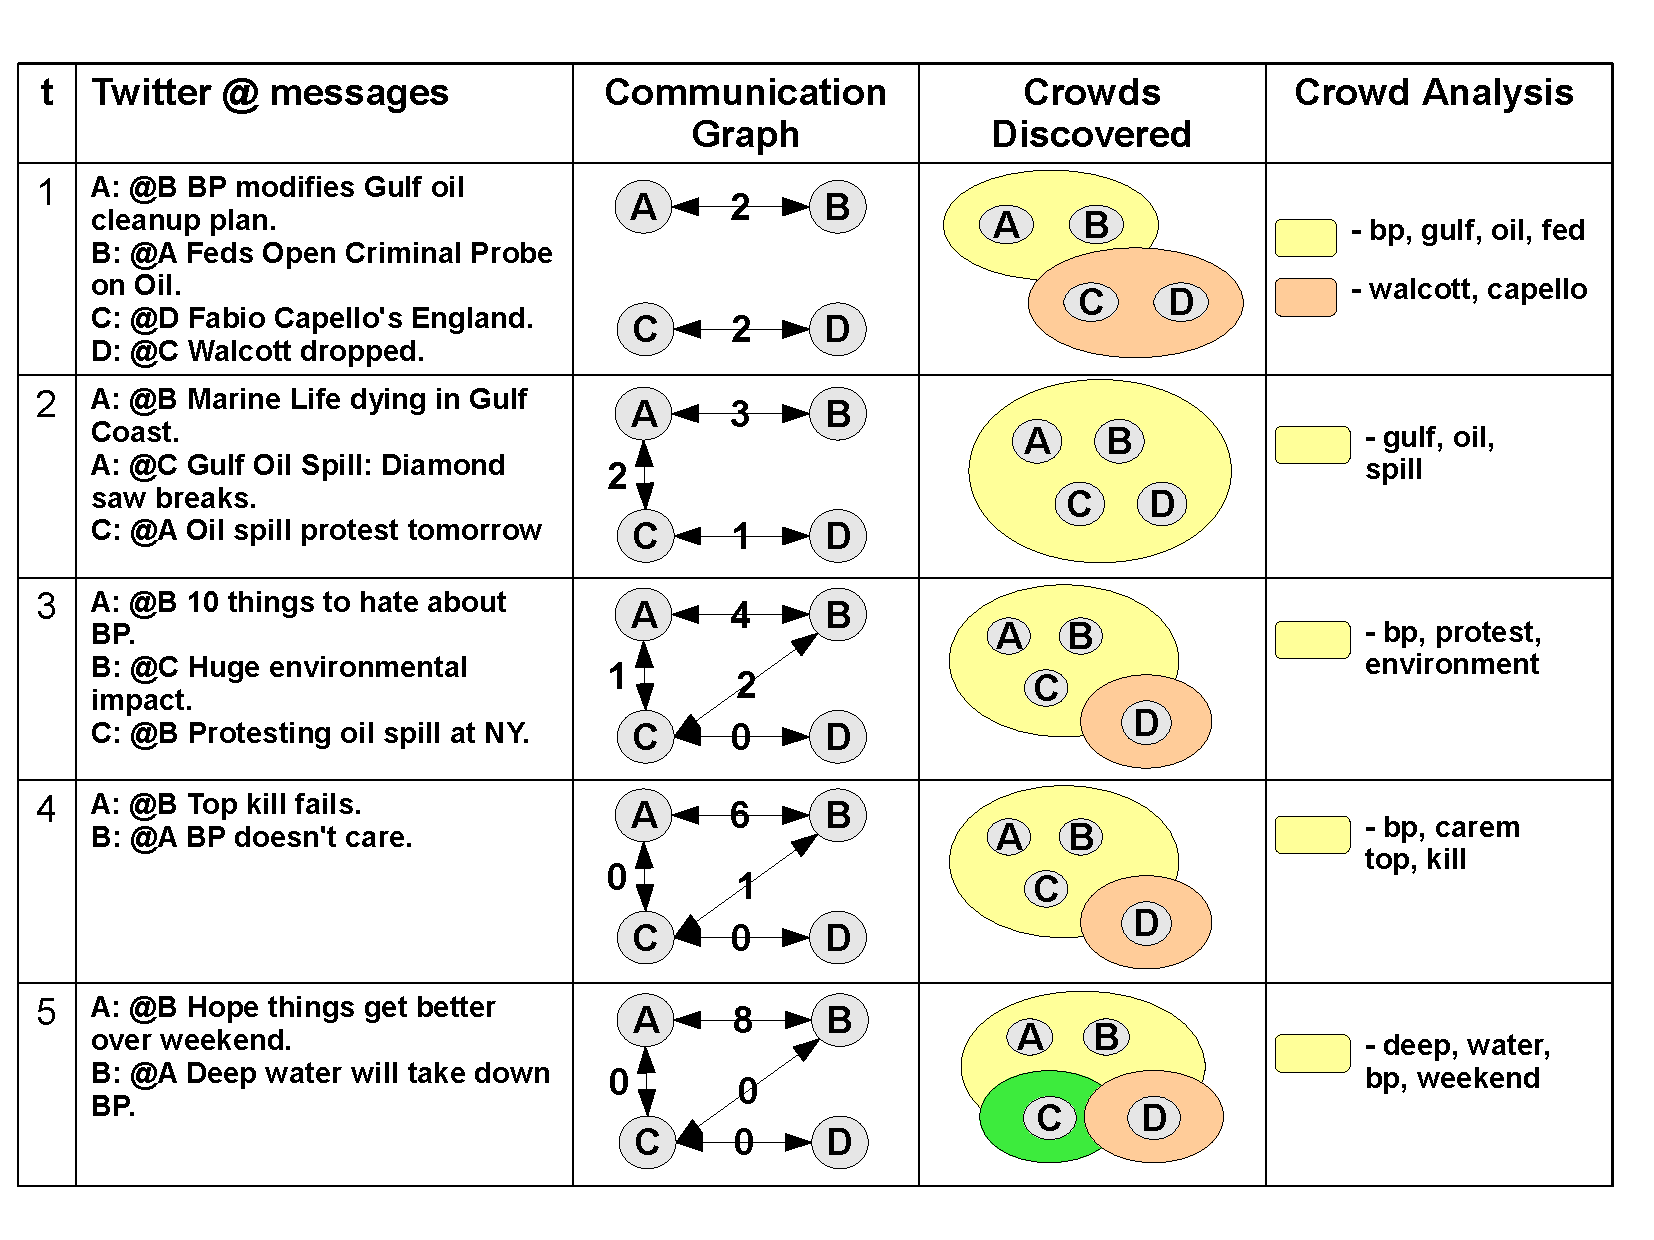
\includegraphics[width=\linewidth]{images/intro}
\caption{Example of crowd discovery and tracking in Twitter.}
\label{fig:intro-example}
\end{figure}
To illustrate the problem of crowd discovery, consider the simple example in
Figure~\ref{fig:intro-example}. At time t=1, users A and B send messages to each
other, as do users C and D.\footnote{For simplicity, the example discretizes
time so that all messages between users occur in steps. In practice, the proposed
algorithm relaxes this assumption and can handle arbitrary message sending
times.} The associated communication graph shows an edge between the two pairs,
where for simplicity the edge is annotated with the number of messages between
the users (2, in both cases). Further, suppose we identify crowds based purely on
graph connectivity. So for time t=1, we see there are two crowds discovered
\{A,B\} and \{C,D\}. For each crowd, we can characterize the semantics of their
communication with simple keywords extracted from the content of the tweets:
(``oil'', ``gulf'') and (``walcott'', ``capello''). At time t=2, the
communication graph is updated with a new edge (connecting User A and User C),
and the existing edges are decayed by one (again, a simplifying assumption for
the purposes of this example). A single crowd is discovered since all users are
connected via edges with non-zero edge weights. At time t=3, User D leaves the
main crowd since no messages to or from User D have been observed since time t=1.
This process continues until time t=5 when User C also leaves the main crowd due
to inactivity. Note that crowds are discovered from communication graph only and
not from the content of the messages. As an example of crowd tracking, we can
track the evolution of the yellow crowd across time periods, observing the
changes it goes through as it grows in size from t=1 to t=2 and then reduces to
two users by t=5.

The grouper deals with the transient crowd discovery and tracking in systems like Facebook and Twitter. For practical crowd discovery and tracking in a large time-evolving communication network, however, we face four key challenges:

\begin{list}{\labelitemi}{\leftmargin= 0.3cm}

\item First, systems like Facebook and Twitter are extremely large (on the order
of 100s of millions of unique users), placing huge demands on the computational
cost of traditional community detection approaches (which can be $O(n^3)$ in the
number of users \cite{flake:cut-clustering}).

\item Second, these services support a high-rate of edge addition (new
messages) so the discovered crowds may become stale quickly, resulting in the need to
re-identify all crowds at regular intervals (again, incurring the high cost of
community detection). The bursty nature of user communication demands a crowd
discovery approach that can capture these highly-temporal based clusters.

\item Third, the strength of association between two users may depend on many
factors (e.g., recency of communication), meaning that a crowd discovery approach
based on graph clustering should carefully consider edge weights. With no decay
at all (meaning that edges are only inserted into the network but never removed),
all users will tend towards a single trivial large crowd. Conversely, overly
aggressive edge decay may inhibit any crowd formation at all (since edges between
users may be removed nearly as soon as they are added).

\item Fourth, crowds may evolve at different rates, with some evolving over
several minutes, while others taking several days. Since crowds are inherently
ad-hoc (without unique community identifiers -- e.g., Fans of LA Lakers), the
formation, growth and dispersal of crowds must be carefully managed for
meaningful crowd analysis.
\end{list}

With these challenges in mind, we propose to discover and track transient crowds
through a communication based clustering approach over time-evolving
graphs that captures the natural conversational nature of social messaging
systems. Two of the salient features of the proposed approach are (i) an
efficient locality-based clustering approach for identifying crowds of users in
near real-time compared to more heavyweight static clustering algorithms; and
(ii) a novel crowd tracking and evolution approach for linking crowds across time
periods.

To support transient crowd discovery in Twitter-like services with 100s of
millions of participants, we propose to leverage the inherent locality in social
messaging systems. Concretely, we identify two types of locality that are
evident in Twitter-like messaging systems: (i) temporal locality and (ii) spatial
locality.

\medskip \noindent\textbf{Temporal Locality:} Transient crowds are
intuitively short-lived, since they correspond to actively communicating groups
of users. Hence, the composition of a crowd at a point-in-time should be impacted
by recent messages as opposed to older messages. As more users interact with the
crowd, the crowd should grow reflecting this \textit{temporal locality} and then
shrink as users in the crowd become inactive (that is, their last communication
with the crowd becomes more distant in time).

\medskip \noindent \textbf{Spatial Locality:} Intuitively, transient crowds are
made up of a very small percentage of users compared to the entire population of
the social network. Hence, new messages (corresponding to the addition of edges
to the communication network) should have only a local influence on the crowds
that exist at any given time. That is, changes in a small region of a graph
should not affect the entire graph. In a dataset of 61 million Twitter messages
described in \cite{Kamath:2011:TCD}, we have confirmed the existence of
this \textit{spatial locality} by finding that only about 1\% of users are within
two hops, meaning that an edge insertion has only a local effect.

\medskip Hence, we can take advantage of both, local changes to the overall
communication network (spatial locality) and recent changes to the network
(temporal locality), for supporting efficient transient crowd discovery. The complete algorithm is described in \cite{Kamath:2011:TCD}

\subsection{Sample Crowds Discovered}
\begin{figure}[!t]
\centering
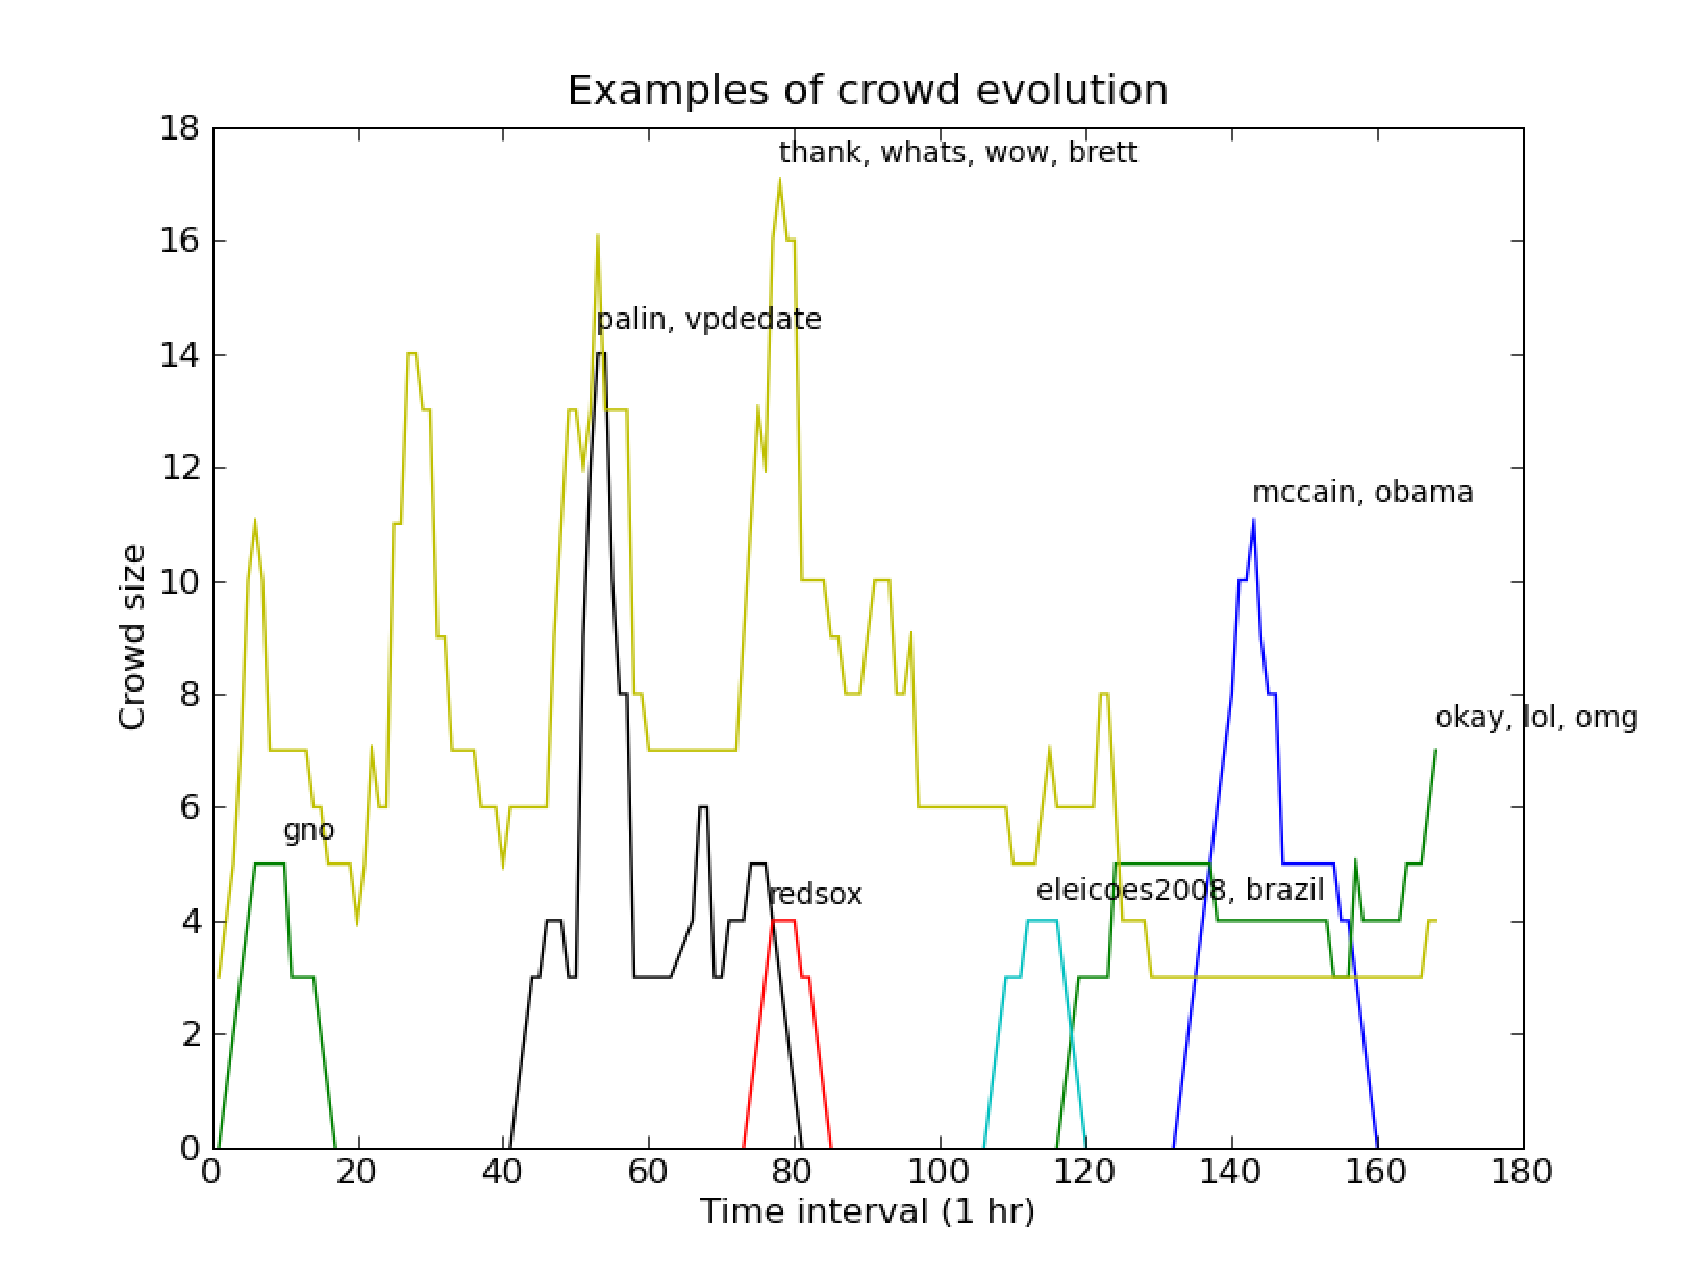
\includegraphics[width=\linewidth]{images/clusterExamplesOverTime}
\caption{Examples of the crowds discovered in the dataset.}
\label{fig:cluster-example}
\end{figure}
We illustrate
some of the discovered crowds and their lifespans in
Figure~\ref{fig:cluster-example}, with an annotation next to the crowd peak
showing the topic of discussion. We see a crowd (shown in black)
discussing Sarah Palin and the Vice-Presidential debate from the $40^{th}$ hour
to $80^{th}$ hour that peaks around the time of the actual debate. We
observe that crowds that talk about general everyday things have a greater
lifespan than crowds discussing specific events. For example in
Figure~\ref{fig:cluster-example}, a crowd (annotated with \textit{thank, whats,
wow}) discussing everyday things lives through the entire week, while, during the
same period we observe several event-specific crowds, like crowds discussing the
Red Sox, Sarah Palin, and Girl's Night Out (gno) forming and dispersing. These
event-specific crowds start forming just before the event and die a few intervals
after the completion of that event. This distinction between the crowds
discovered clearly indicates two types of Twitter usage: first, it is used as a
platform to discuss and debate specific events, and second, it as also used a means of
everyday communication.

\section{Architecture}
\label{sec:architecture}
\begin{figure}[!t]
\begin{center}
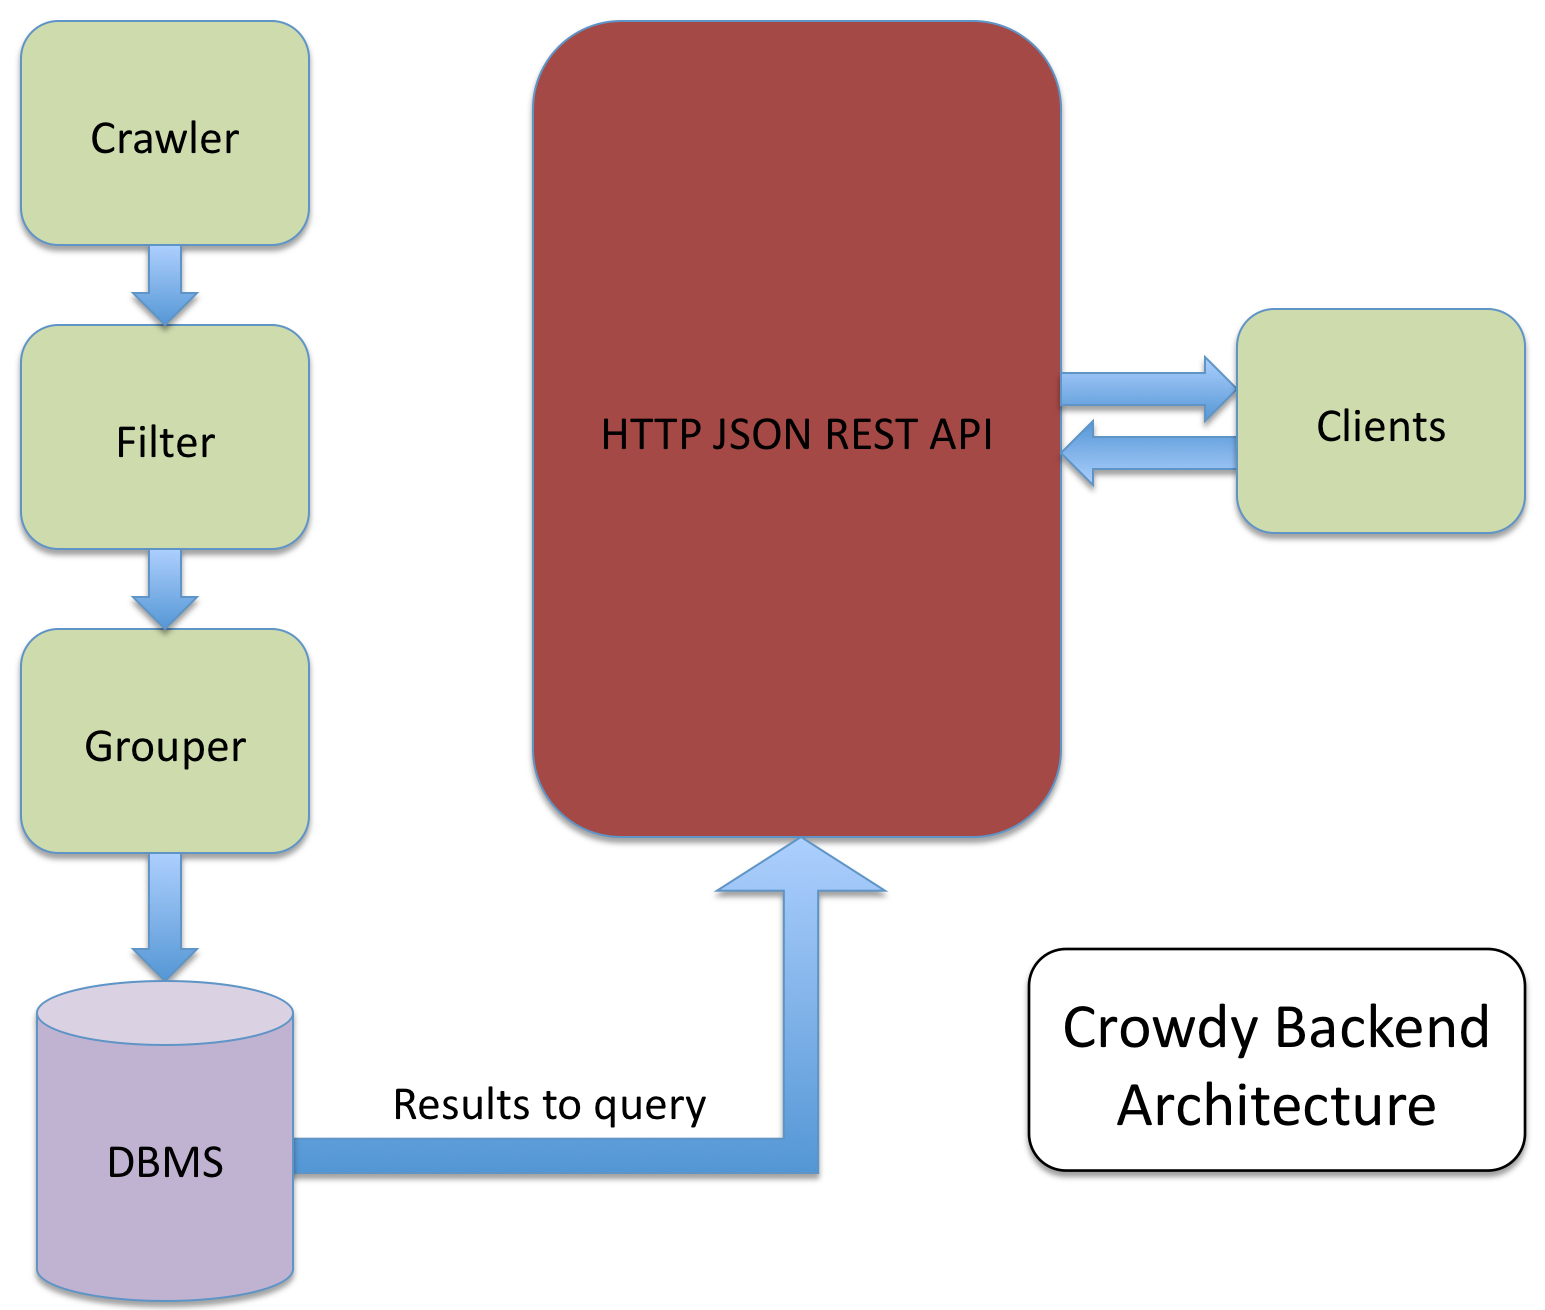
\includegraphics[width=3.0in]{images/architecture}
\caption{Examples for trending phrases discovery problem.}
\label{fig:candidate_phrases}
\end{center}
\end{figure}

An architecture for our solution is shown in Figure 1.  Data flows from a
crawler, through zero or more filters, to a grouper, and then through zero or
more filters, and then it is finally stored in a MongoDB database.  We went
with an extremely modular architecture to make the system flexible.  We can
easily integrate new crawlers, filters, and groupers into the system.The
various modules of this architecture are described in the remainder of this
section.

\subsection{Crawler}
Crawlers interact with social media websites to collect information. All of the
crawlers we use in this project acquire tweets and users from Twitter using
their APIs.

\subsubsection{Localcrawl}
This crawler collects data from users
in a region using the standard Twitter API. We started with a tiny sample set
of seed users. It uses snowball sampling to collect more users that are likely
to live in an area. Once we have a list of users 

We have used this crawler and the crowd detection algorithms on both Bryan/College
Station and the Houston area, but the demo is currently exclusively running on the
Bryan/College Station data.

\subsubsection{GeoStream}
This crawler listens to Twitter's
streaming API to find geo-located tweets.  It receives every geo-located tweet
posted from anywhere in the world.  In the future, this data may be used to
show crowds on a map.

\subsection{Grouper}
Groupers detect crowds in the data collected by a crawler.  The precise
definition of a crowd depends on the implementation of the grouper.  A grouper
could create crowds based on communication patterns, geographical proximity, or
textual similarity. Once crowds are discovered, this module formats crowds to a
well defined crowds object and adds it to a DBMS.

\subsubsection{Mentions}
For this project, we exclusively discover crowds based on communication.  The
mentions grouper looks for sets of people who are communicating with each
other.  The algorithm to discover crowds is described in
Section~\ref{sec:crowd_algorithm}.

\subsection{Filter}
Filters are used to remove unnecessary data, such as spam tweets, and add
automatically generated metadata to tweets, users, and crowds.  A filter can
appear before or after the grouper module as needed.  In the following
sections, we discuss two filters that we implemented and several that we plan
to add in the future.

\subsubsection{Lucene Filter}
The Lucene module creates a Lucene index from the text of the tweets in a
crowd.  This index is used to speed up searching through the text of the
tweets. This filter is designed so that a crowd can be updated as new data
arrives from a crowd.

\subsubsection{Network Filter}
We also have a network filter that builds a graph that represents the
communication between the users in a crowd. At the moment, it analyzes two things:
degree centrality and clustering coefficient.  The degree centrality is used to
find the most important users in a given crowd. The clustering coefficient of
the crowd is added to the crowd as automatically generated metadata 

\subsubsection{Planned Filters}
There are several filters that we have not implemented, but may implement in
the future. The ability to easily add new filters and create an automated
workflow is an important part of our design.
\begin{itemize}
\item Remove users that appear to be spammers.
\item Add metadata to each user that contains an estimate of the users
    location, and some information about the quality of the estimate.
\item Find the key terms in a crowd and add that metadata to the crowd.
\item Summarize the tweets from a crowd.
\end{itemize}

\subsection{HTTP JSON RESTful APIs}: This module provides client an interface to the digital library. The module exposes JSON APIs that the clients can use to browse and search the crowds archive. Here is a brief description of the more important methods:
\begin{description}
 \item[search/crowd] Find crowds sorted by relevance or time.
 \item[crowd/id] Retrieve all of the data for a crowd.
 \item[crowd/users] Retrieve a list of all the users in the crowd.
 \item[crowd/tweets] Retrieve a list of all the tweets in the crowd.
 \item[crowd/star] Mark a crowd as significant.
 \item[user/edges] Retrieve the friend and follower relationships for a given user.
\end{description}

\subsection{Tools}

The tool we used to develop this framework are as follows:
\begin{itemize}
 \item \noindent\textbf{PyLucene}: To provide the search functionality we use Apache Lucene. It provides methods for text indexing and searching. To integrate Lucene with our framework we use Pylucene which is a Python wrapper for Lucene. This is used in the filter module of our architecture.
 \item \noindent\textbf{CherryPy}: This is an object-oriented web framework for Python. The JSON REST API that interface the digital library with clients is hosted using this web framework.
 \item \noindent\textbf{NetworkX}: This is a library for manipulating graphs in Python. We use this to determine quality of crowds generated by crowd detection framework and filter out crowds of poor quality. This sits in the filter module.
  \item \noindent\textbf{Beanstalk}: Beanstalk is a simple, fast work queue. We use it to connect the crawlers, filters, and groupers together.
   \item \noindent\textbf{MongoDB}: MongoDB is a scalable, high-performance, open source, document-oriented database. We store the crowds discovered by the framework in this DB. The API module interacts with this database to retrieve collections as required by the user query.
\end{itemize}

\section{Conclusion}
\label{sec:conclusion}
In this project, we presented a framework of a digital library for transient crowds in highly-dynamic social messaging systems like Twitter and Facebook. We built a framework that allows an analyst or curious user to find interesting crowds and see how they evolve.  The framework enabled clients to interact with the library using JSON APIs. The APIs enabled searching and browsing of the digital library.

{
 \bibliographystyle{abbrv}
 \bibliography{sigproc}
}
\balancecolumns % GM July 2000

\end{document}
